\paragraph{В четвертой} главе приводится имитационное моделирование развиваемых алгоритмов. В качестве алгоритма
для сравнения используется параллельный коррелятор с алгоритмом уточнения частоты.

Алгоритм оценки параметров ШПС в условиях интерференции (Delay and Multiply Approach + уточненный АР).
В работе предлагается объединить результаты работы алгоритма Delay and Multiply Approach и, предложенных
в данной работе, усовершенствованного итеративного алгоритма уточнения АКФ гармонического
сигнала и подхода для оценки частоты широкополосного сигнала при помощи АР-модели.

Схематично приемник изображен на рисунке \ref{pic:ar_dma_scheme}.

\begin{figure}[H]
\center\scalebox{1}{\includegraphics[width=1\linewidth]{dma_quadruple_lpc.eps}}
	\caption{Алгоритм обнаружения и оценки параметров ШПС в условиях интерференции (DMA + уточненный АР)}
	\label{pic:ar_dma_scheme}
\end{figure}

Выходом алгоритма Delay  является оценка фазы ПСП. Повторно модулируя входящий сигнал ПСП с полученной
фазой, можно восстановить гармонический сигнал. Для оценки частоты данного сигнала применяется
АР-метод. Но для оценки АР-методом, требуется точная оценка АКФ, которую можно получить
с помощью усовершенствованного итеративного алгоритма вычисления АКФ.

{\underline{Предложенный алгоритм можно описать следующим набором шагов:}}
\begin{itemize}
\item[Шаг 1.] Входной сигнал ${x(m)}$ умножается на задержанную копию ${x(m-\tau)}$. Так же
	на данном шаге можно производить когерентное накопление результата, для
	увеличения ОСШ.

	\begin{center}
	\begin{equation}
		%\label{}
		x_{new}(m) = \frac{C_{new}(k)}{2} \left(\cos (2\pi f \tau) - \cos \left[2 \pi f (2m - \tau)\right]\right)
	\end{equation}
	\end{center}

\item[Шаг 2.] Полученный сигнал ${x_{new}(m)}$ фильтруется ФНЧ для отсечения высокочастотной компоненты.
\item[Шаг 3.] Генерируется локальная ПСП ${C(m)}$ и умножается на задержанную копию ${C(m-\tau)}$.

	\begin{center}
	\begin{equation}
		%\label{}
		C_{new}(m) = C(m)C(m-\tau)
	\end{equation}
	\end{center}

\item[Шаг 4.] Отфильтрованный сигнал ${x_{filt}(m)}$ коррелируется с новой ПСП ${C_{new}(m)}$
	с использованием БПФ. Выход коррелятора сравнивается с заранее определенным порогом.

	\begin{center}
	\begin{equation}
		%\label{}
		x_{filt}(m) = \frac{C_{new}(m)}{2} \cos (2\pi f \tau)
	\end{equation}
	\end{center}

	\subitem{\underline{Если}}  значение оказалось больше порогового {\underline{то}},
		принимается решение о наличии сигнала. Полученное значение фазы ПСП  - ${k}$ запоминается.
		Перейти на шаг 5.
	\subitem{\underline{Иначе}} 
		Выбирается ${N}$ максимальных значений и запоминаются их фазы ПСП.
\item[Шаг 5.] Входной сигнал ${x(m)}$ модулируется ПСП ${C(m-k)}$, где ${k}$ - это фаза ПСП из ${N}$ - выбранных. В результате получаем гармонический
	сигнал ${x_{cos}(m)}$ с неизвестной частотой.
\item[Шаг 6.] Для увеличения ОСШ сигнала ${x_{cos}(m)}$ вычисляется значение уточненное значение АКФ
	по усовершенствованному итеративному алгоритму получения АКФ.
\item[Шаг 7.] Определяются коэффициенты АР-модели ${\hat{a_1}, \hat{a_2}}$.
	Вычисляется резонансная частота ${\omega_1}$ и определяется квадрат модуля частотного отклика АР-модели для этой частоты. 
\item[Шаг 8.]
	Сравнение квадрата модуля с порогом.
        \subitem{\underline{Если}}  значение оказалось больше порогового {\underline{то}} 
                принимается решение о наличии сигнала, а в качестве оценки
                частоты принимается значение ${\omega_1}$ соответствующее выбранной фазе ПСП. 
        \subitem{\underline{Иначе}} 
		\subsubitem\underline{Если} остались непроверенные фазы ПСП - переход на шаг 5.
		\subsubitem\underline{Иначе} сигнал не обнаружен.
\end{itemize}

Общее количество умножений, необходимых для детектирования и оценки частоты от одного источника предлагемым
алгоримом (количество итераций в алгоритме уточнения АКФ ${k=3}$): ${OP_{DMA\_ACF\_AR} = 16NlogN + 11N + 51}$.

Количество итераций требуемых для оценки частоты одного источника параллельным корррелятором:
${OP_{corr} = 48NlogN + 65N}$.

Предлагаемый подход существенно выигрывает по вычислительным затратам в сравнении с параллельным коррелятором.
